\documentclass[pdflatex,compress]{beamer}

%\usetheme[dark,framenumber,totalframenumber]{ElektroITK}
\usetheme[darktitle,framenumber,totalframenumber]{ElektroITK}
\usepackage{graphicx}
\usepackage{multicol}

\title{Data Communications}
\subtitle{Chapter 1 - Introduction}

\author{Mifta Nur Farid}

\begin{document}

\maketitle

\begin{frame}
	\title{Technological Advancement Driving Forces}
	\begin{center}
		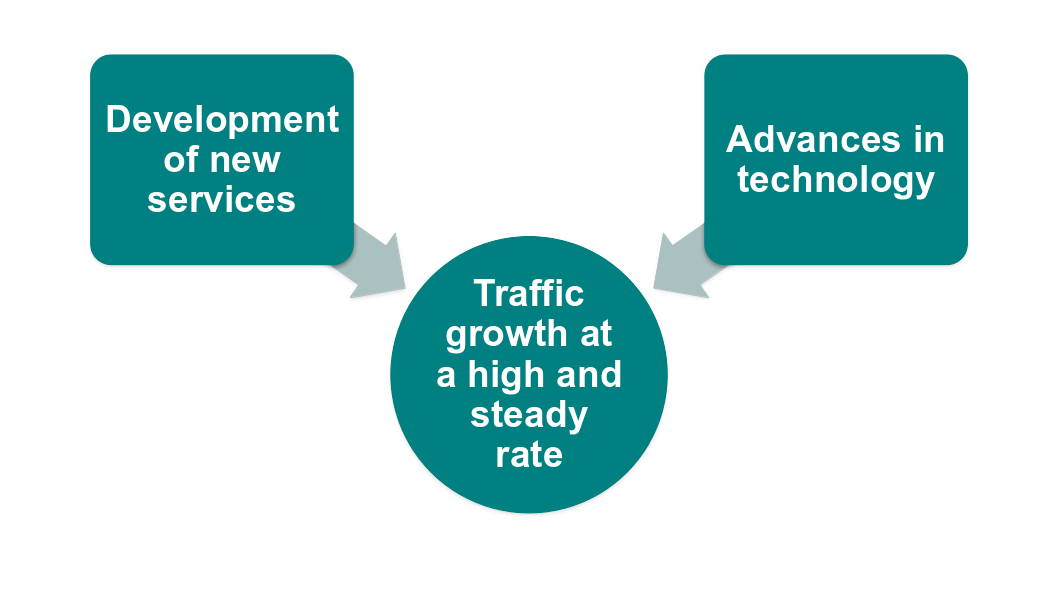
\includegraphics[width=\linewidth]{img/img01}
	\end{center}
\end{frame}

\begin{frame}
	\begin{center}
		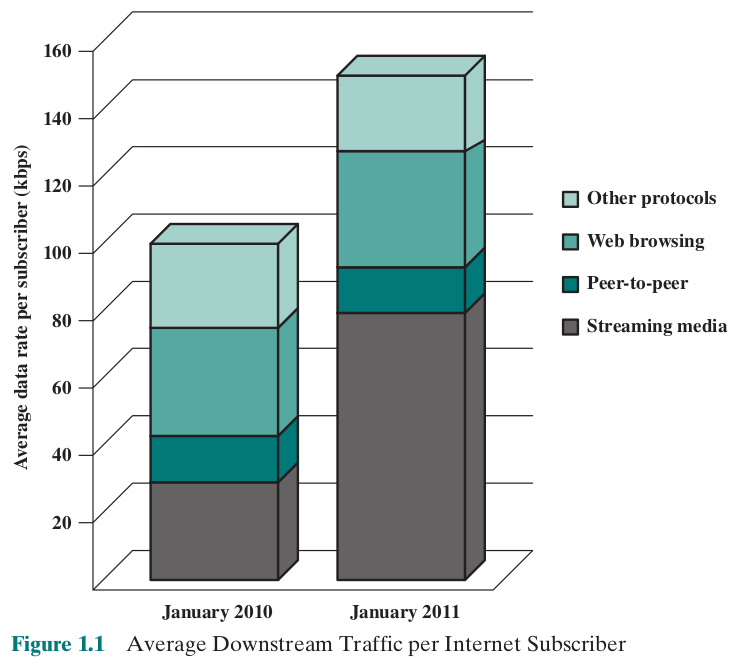
\includegraphics[height=0.8\textheight]{img/img02}
	\end{center}
\end{frame}

\begin{frame}
	\frametitle{Notable Trends}
	\begin{enumerate}
		\item \textbf{Trend toward faster and cheaper, in both computing and communication}
		\begin{itemize}
			\item More powerful computers supporting more demanding applications
			\item The increasing use of optical fiber and high-speed wireless has brought transmission prices down and greatly increased capacity
		\end{itemize}
		\item \textbf{Today's networks are more "intelligent"}
		\begin{itemize}
			\item Differing levels of quality of service (QoS)
			\item Variety of customizable services in the areas of network management and security
		\end{itemize}
	\end{enumerate}
\end{frame}

\begin{frame}{Notable Trends}
	\begin{enumerate}
		\setcounter{enumi}{2}
		\item \textbf{The Internet, the Web, and associated applications have emerged as dominant features for both business and personal network landscapes}
		\begin{itemize}
			\item "Everything over IP"
			\item Intranets and extranets are being used to isolate proprietary information
		\end{itemize}
		\item \textbf{Mobility}
		\begin{itemize}
			\item iPhone, Droid, and iPad have become drivers of the evolution of business networks and their use
			\item Enterprise applications are now routinely delivered on mobile devices
			\item Cloud computing is being embraced
		\end{itemize}
	\end{enumerate}
\end{frame}

\begin{frame}
	\begin{center}
		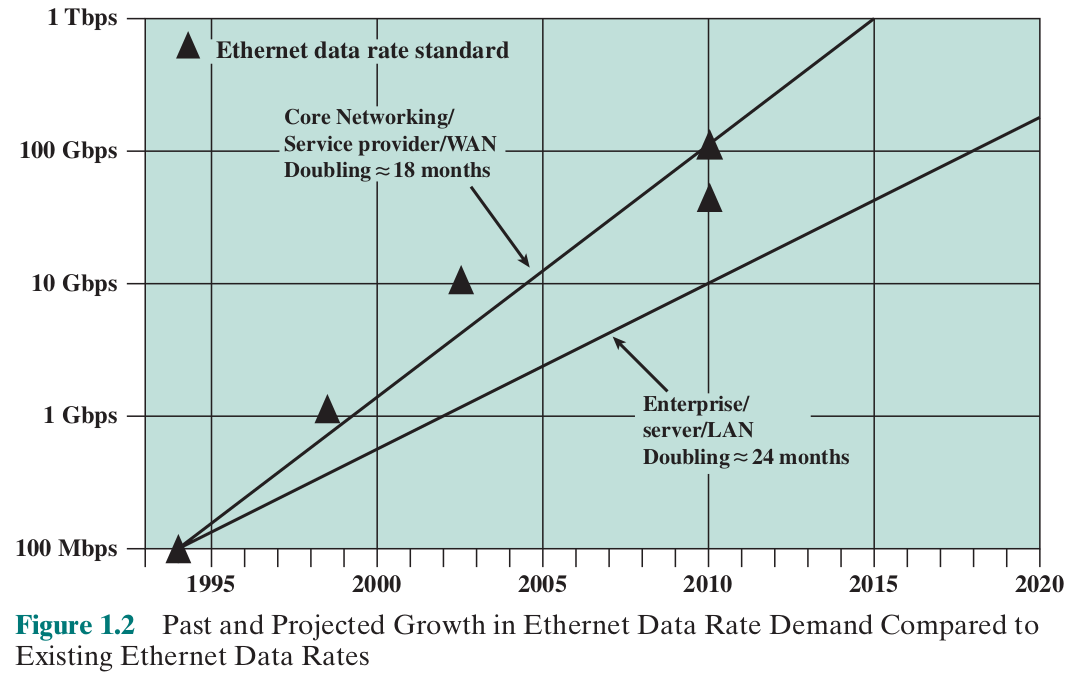
\includegraphics[height=0.8\textheight]{img/img03}
	\end{center}
\end{frame}

\begin{frame}
	\frametitle{Changes in Networking Technology}
	\begin{itemize}
		\item \textbf{Emergence of high-speed LANs}
		\item \textbf{Corporate WAN needs}
		\item \textbf{Digital electronics}
	\end{itemize}
\end{frame}

\begin{frame}
	\frametitle{Emergence of High-Speed LANs}
	\begin{itemize}
		\item Personal computers and microcomputer workstations have become an essential tool for office workers
		\begin{center}
			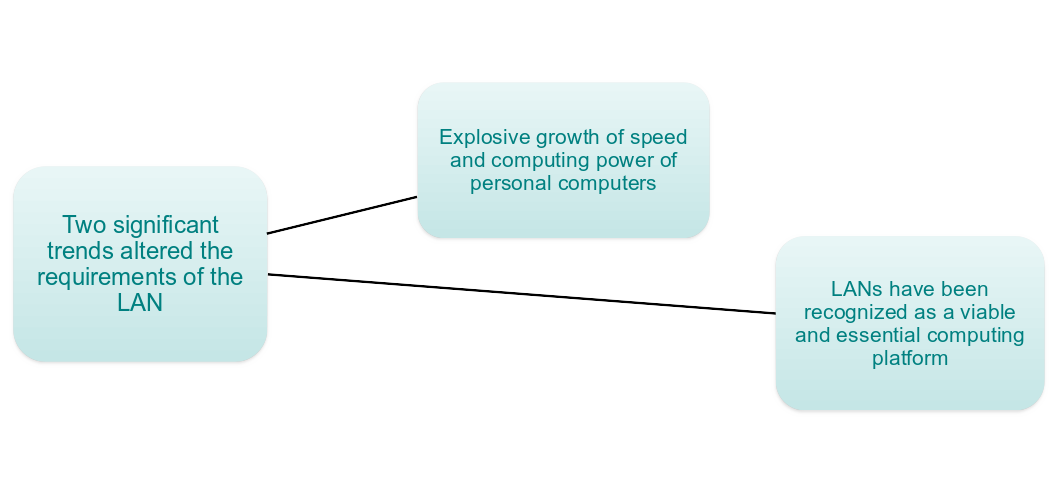
\includegraphics[height=0.5\textheight]{img/img04}
		\end{center}
		\item Examples of requirements that call for higher- speed LANs:
		\begin{itemize}
			\item Centralized server farms
			\item Power workgroups
			\item High-speed local backbone
		\end{itemize}
	\end{itemize}
\end{frame}

\begin{frame}
	\frametitle{Corporate Wide Area\\Networking Needs}
	\textbf{Changes in corporate data traffic patterns are driving the creation of high-speed WANs}
	\begin{itemize}
		\item Growing use of telecommuting
		\item Nature of the application structure has changed
		\item Intranet computing
		\item More reliance on personal computers, workstations, and servers
		\item More data-intensive applications
		\item Most organizations require access to the Internet
		\item Traffic patterns have become more unpredictable
		\item Average traffic load has risen
		\item More data is transported off premises and into the wide area
	\end{itemize}
\end{frame}

\begin{frame}
	\frametitle{Digital Electronics}
	\begin{itemize}
		\item The rapid conversion of consumer electronics to digital technology is having an impact on both the Internet and corporate intranets
		\begin{itemize}
			\item Image and video traffic carried by networks is dramatically increasing
			\begin{itemize}
				\item Because of their huge storage capacity digital versatile disks (DVDs) are being incorporated into Web sites
				\item Digital camcorders have made it easier to make digital video files to be placed on corporate and Internet Web sites
			\end{itemize}
		\end{itemize}
	\end{itemize}
\end{frame}

\begin{frame}
	\frametitle{Convergence}
	\begin{itemize}
		\item The merger of previously distinct telephony and information technologies and markets
		\begin{itemize}
			\item Involves:
			\begin{itemize}
				\item Moving voice into a data infrastructure
				\item Integrating all the voice and data networks inside a user organization into a single data network infrastructure
				\item Then extending that into the wireless arena
			\end{itemize}
			\item Foundation is packet-based transmission using the Internet Protocol (IP)
			\item Increases the function and scope of both the infrastructure and the application base
		\end{itemize}
	\end{itemize}
\end{frame}

\begin{frame}
	\frametitle{Convergence}
	\begin{center}
		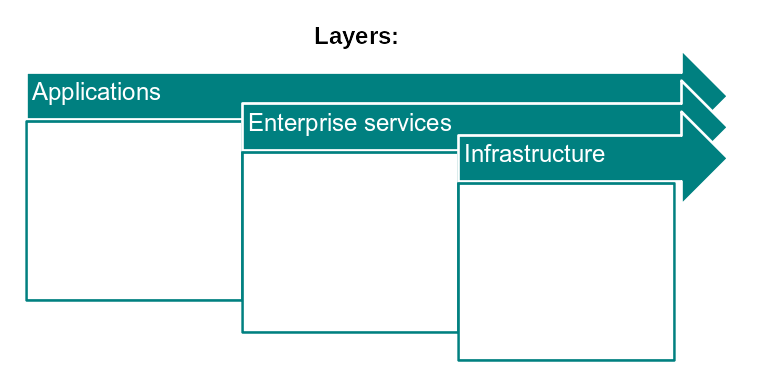
\includegraphics[width=\linewidth]{img/img05}
	\end{center}
\end{frame}

\begin{frame}
	\frametitle{Communications Model}
	\begin{center}
		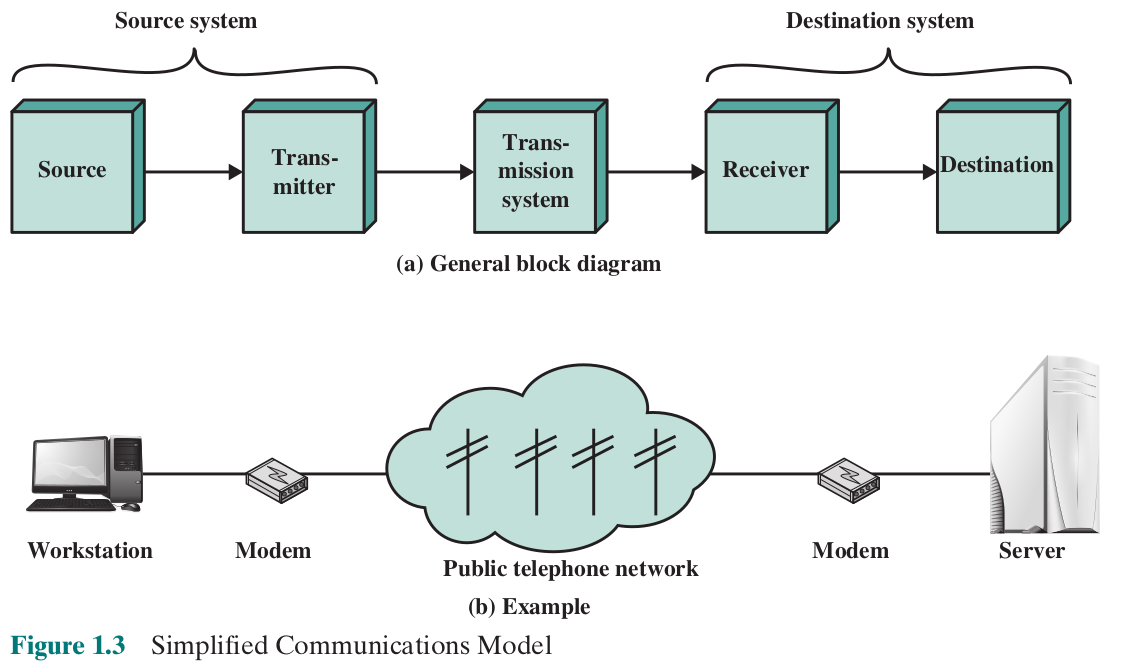
\includegraphics[width=\linewidth]{img/img06}
	\end{center}
\end{frame}

\begin{frame}
	\begin{center}
		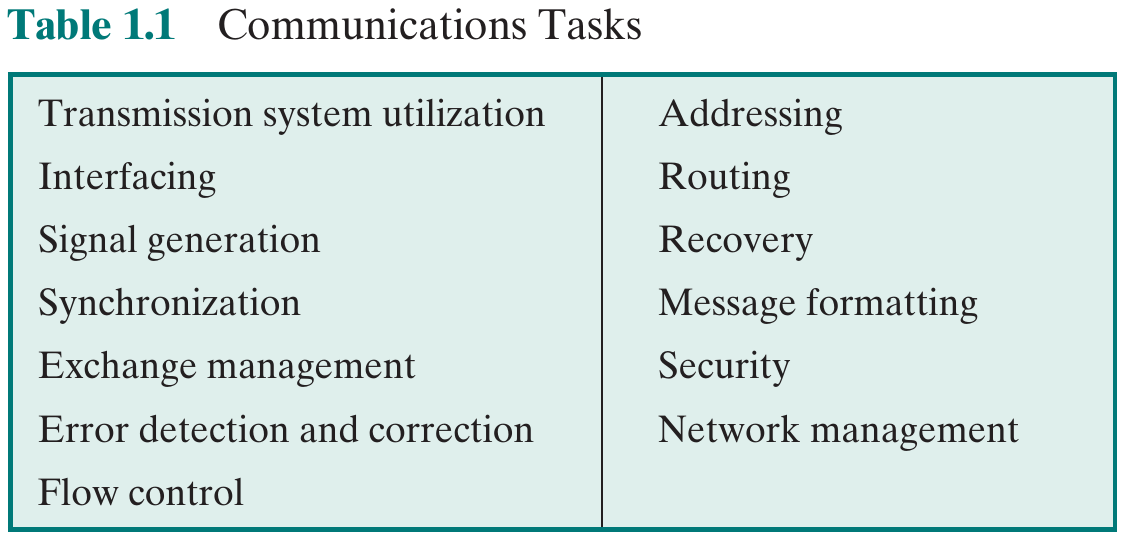
\includegraphics[width=\linewidth]{img/img07}
	\end{center}
\end{frame}

\begin{frame}
	\begin{center}
		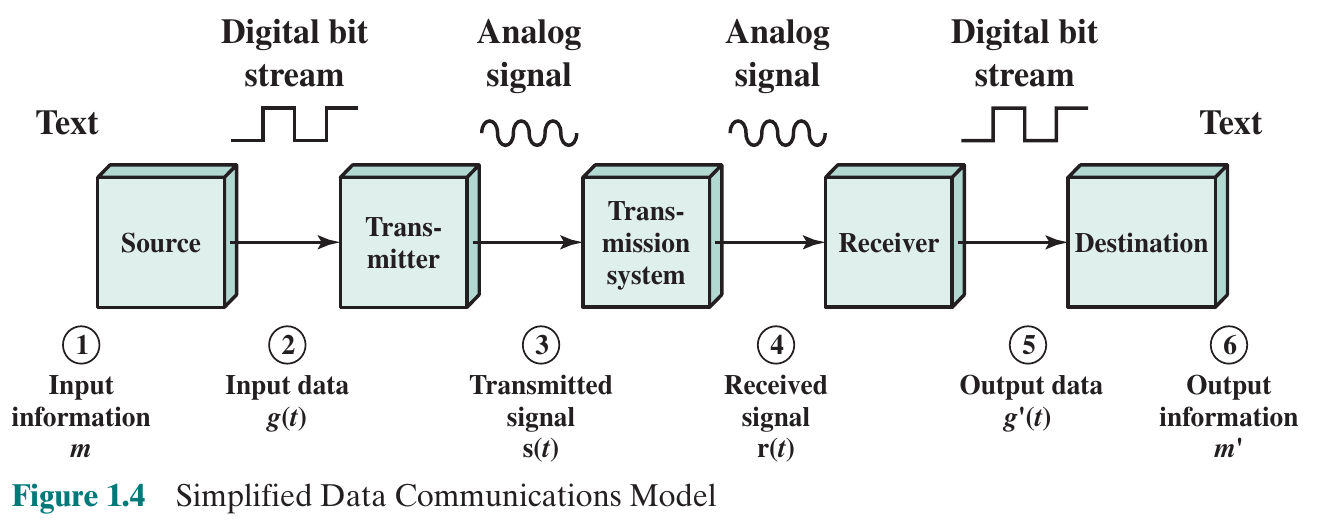
\includegraphics[width=\linewidth]{img/img08}
	\end{center}
\end{frame}

\begin{frame}
	\frametitle{Transmission Lines}
	\begin{multicols}{2}
		\begin{itemize}
			\item The basic building block of any communications facility is the transmission line
			\item The business manager is concerned with a facility providing the required capacity, with acceptable reliability, at minimum cost
		\end{itemize}		
		\columnbreak
			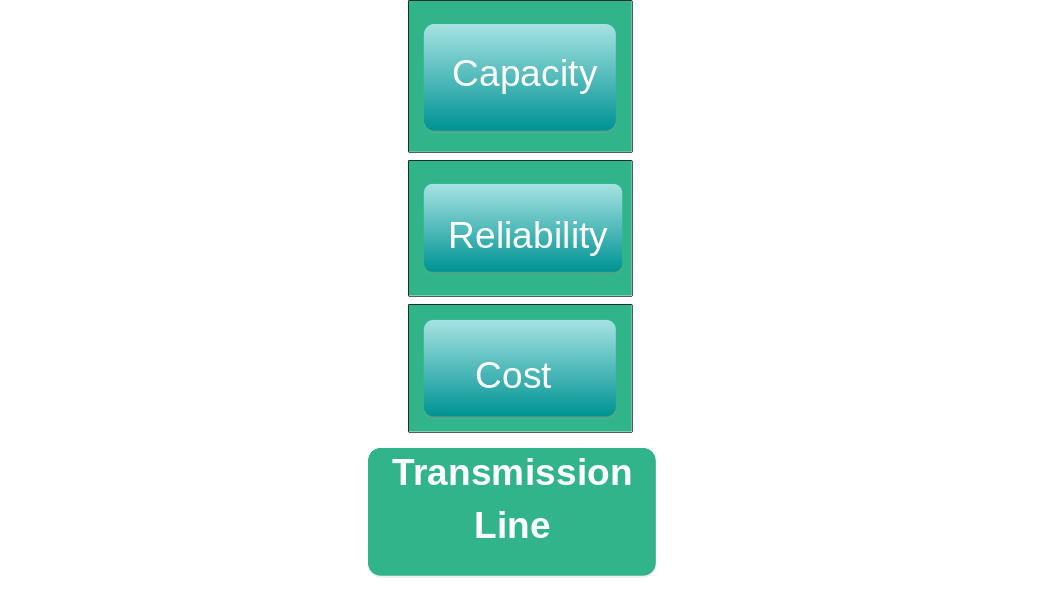
\includegraphics[width=1.5\linewidth]{img/img09}
	\end{multicols}
\end{frame}

\begin{frame}
	\frametitle{Transmission Mediums}
	Two mediums currently driving the evolution of data communications transmission are:
	\begin{enumerate}
		\item Fiber optic transmissions
		\item Wireless transmissions
	\end{enumerate}
\end{frame}

\begin{frame}
	\frametitle{Transmission Services}
	\begin{itemize}
		\item Remain the most costly component of a communications budget
		\item Two major approaches to greater efficiency:
		\begin{multicols}{2}
			\centering \textbf{Multiplexing}\\
			\centering The ability of a number of devices to share a transmission facility\\
			\columnbreak
			\centering \textbf{Compression}\\
			\centering Squeezing the data down so that a lower-capacity, cheaper transmission facility can be used
		\end{multicols}
	\end{itemize}
\end{frame}

\begin{frame}
	\frametitle{Networks}
	\begin{itemize}
		\item It is estimated that by 2016 there will be over 20 billion fixed and mobile networked devices
		\item This affects traffic volume in a number of ways:
		\begin{itemize}
			\item It enables a user to be continuously consuming network capacity
			\item Capacity can be consumed on multiple devices simultaneously
			\item Different broadband devices enable different applications which may have greater traffic generation capability
		\end{itemize}
	\end{itemize}
\end{frame}

\begin{frame}
	\frametitle{Networking}
	Advances in technology have led to greatly increased capacity and the concept of integration, allowing equipment and networks to work simultaneously
	\begin{center}
		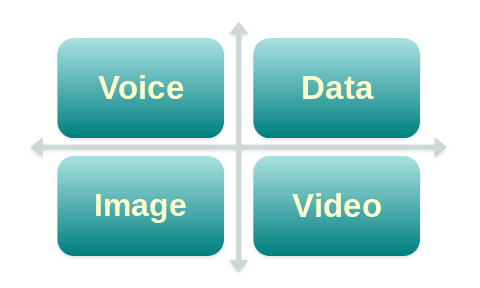
\includegraphics[width=0.5\linewidth]{img/img10}
	\end{center}
\end{frame}

\begin{frame}
	\frametitle{Wide Area Networks (WANs)}
	\begin{itemize}
		\item Span a large geographical area
		\item Require the crossing of public right-of-ways
		\item Rely in part on common carrier circuits
		\item Typically consist of a number of interconnected switching nodes
	\end{itemize}
\end{frame}

\begin{frame}
	\frametitle{Wide Area Networks}
	Alternative technologies used include:
	\begin{itemize}
		\item Circuit switching
		\item Packet switching
		\item Frame relay
		\item Asynchronous Transfer Mode (ATM)
	\end{itemize}
\end{frame}

\begin{frame}
	\frametitle{Circuit Switching}
	\begin{itemize}
		\item Uses a dedicated communications path
		\item Connected sequence of physical links between nodes
		\item Logical channel dedicated on each link
		\item Rapid transmission
		\item The most common example of circuit switching is the telephone network
	\end{itemize}
\end{frame}

\begin{frame}
	\frametitle{Packet Switching}
	\begin{itemize}
		\item Data are sent out in a sequence of small chunks called packets
		\item Packets are passed from node to node along a path leading from source to destination
		\item Packet-switching networks are commonly used for terminal-to-terminal computer and computer-to-computer communications
	\end{itemize}
\end{frame}

\end{document}
